\todo{im prinzip nur aus dem Manifesto abschreiben}
\chapter{Use Cases\label{chap:usecases}}
\begin{figure}[htbp]
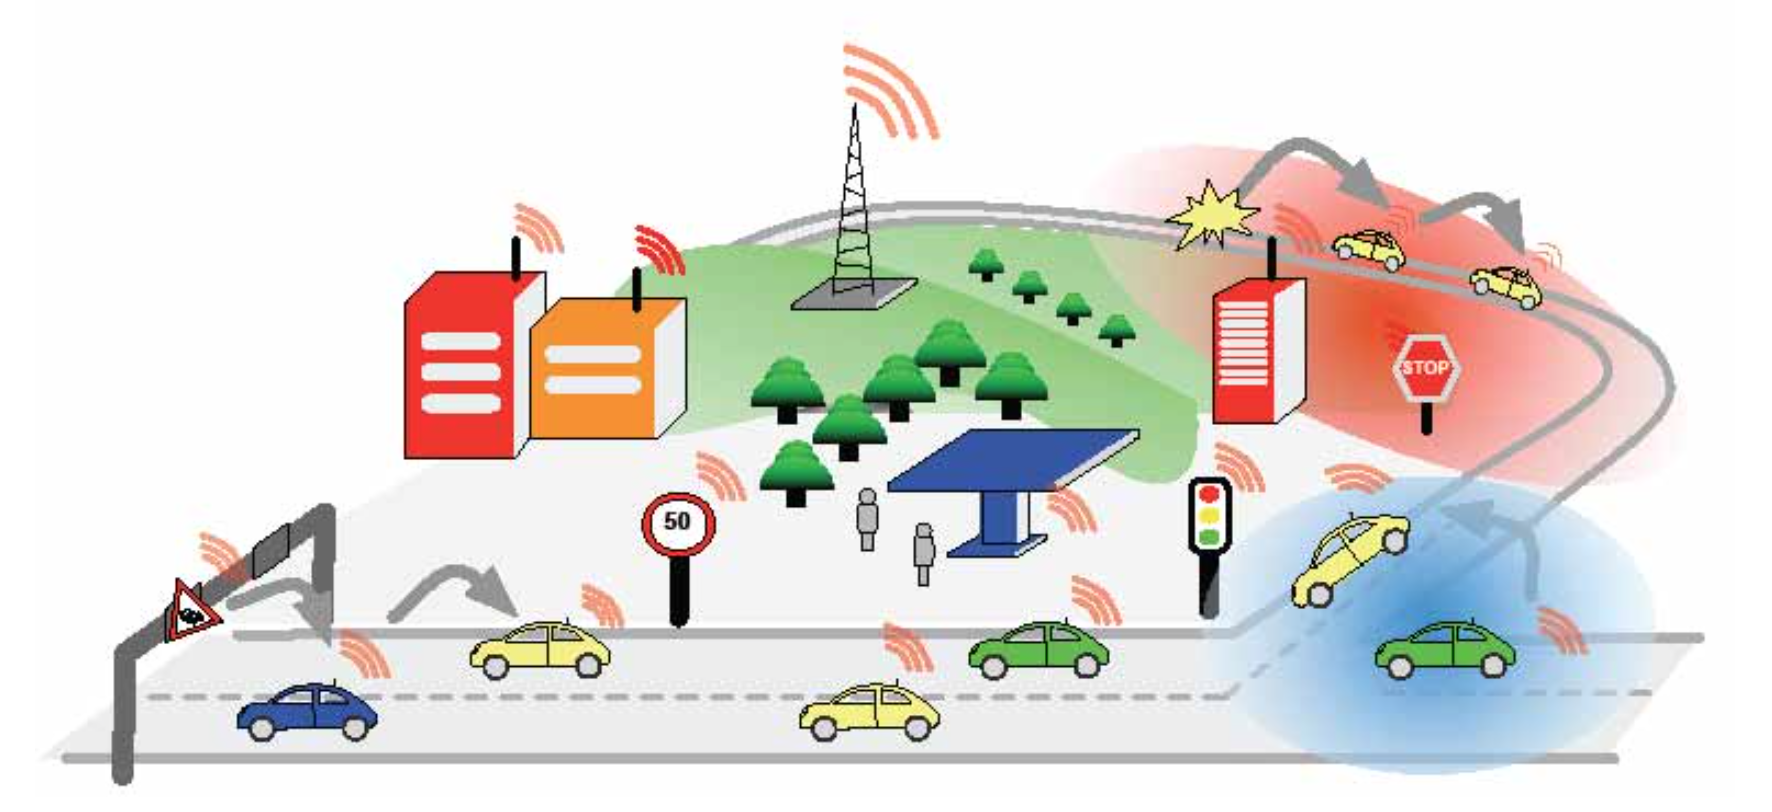
\includegraphics[width=0.99\textwidth]{content/images/06_use_cases/komponenten.png}
\caption{Die Komponenten der \acl{C2C}}
\label{fig:komponentenderc2x}
\end{figure}
Die \acl{C2C} bietet eine große Vielfalt an verschiedenen Einsatzmöglichkeiten. Da es sich bei dem gesamten Projekt nicht nur darum handelt das Fahrzeuge untereinander kommunizieren, sondern wie auf \autoref{fig:komponentenderc2x} zu sehen auch andere Verkehrskomponenten. Hinzu kommt natürlich noch Internet Hotspots die ebenfalls in der C2C eine rolle spielen. Um das Zusammenspiel der Komponenten besser zu verstehen und zu sehen wie groß das Potential der \acl{C2C} ist, werden im folgenden mehrere Szenarien aufgezählt und erklärt. Diese Teilen sich in Sicherheitsbedingte, Verkehrseffiziente und Infotainment ein. 

\section{Sicherheitsbedingt}
Sicherheitsbedingte Szenarien sind Fälle bei denen ein Möglicher Unfall verhindert werden kann. Im Folgenden werden drei Szenarien erklärt bei denen das Unfallrisiko minimiert werden kann.
\subsection{Cooperative Forward Collision Warning}
Einer der häufigsten Ursachen für Verkehrsunfälle sind plötzliche Bremsmanöver von Vorrausfahrenden Fahrzeugen und die Unaufmerksamkeit eines Fahrers. Aus diesen Ursachen besteht ein erhöhtes Risiko für Auffahrunfälle. Cooperative Forward Collision Warning versucht genau dieses Risiko zu vermindern. Um dies zu vollbringen überwacht jedes Fahrzeug die eigenen Informationen, wie die Geschwindigkeit, Richtung und Position und vergleicht diese mit den Daten der anderen Fahrzeugen. Bei Auffälligkeiten und Abweichungen warnt das System dem Fahrer frühzeitig vor einer möglichen Kollision. Diese Warnung kann durch auditive, visuelle oder haptische Alarme signalisiert werden. Da es durchaus sein kann das noch Fahrzeuge, die nicht in dem C2C Netz kommunizieren, unterwegs sind, können über Objekterkennungssensoren diese ebenfalls identifiziert werden. Dadurch sinkt das Risiko noch einmals für die C2C Teilnehmer. Die Informationen werden innerhalb von 20 bis 200 meter geteilt womit auch genug Zeit bleibt um diese Auszuwerten und den Fahrer frühzeitig zu Informieren. 

\subsection{Pre-Crash Sensing/Warning}
Natürlich können nicht alle Unfälle durch die Cooperative Forward Collision Warning vermieden werden. Daher ist davon auszugehen das dennoch Auffahrunfälle geschehen werden. Dafür hat man sich das Pre-Crash Sensing/Warning Szenario ausgedacht, bei dem man von einem Unvermeidbaren Unfall ausgeht. Dies soll durch die \acl{C2C} erkannt und Vorbereitungen für den Unfall getroffen werden. Damit dieses System funktioniert muss wie bei dem vorherigen Szenario dauerhaft Informationen der Fahrzeuge ausgetauscht werden. Dabei geht man davon aus das die Informationen der Fahrzeuge die sich im Umkreis von 20 bis 100 meter befinden überwacht werden müssen. Entdeckt das System einen unvermeidbaren Unfall muss sichergestellt sein das diese Fahrzeuge die Kollidieren werden sicher miteinander kommunizieren können um Daten wie die, Fahrzeuggröße und genaue Position bekannt zu geben. Über diese Informationen können dann Sicherheitsmaßnahmen wie Airbar, Gurtstraffer oder erweiterbare Stoßstangen gesteuert werden und effektiv genutzt werden. 

\subsection{Hazardous Location C2C Notification}
Die Hazardous Location C2C Notification soll dafür sorgen das gefährliche Fahrpassagen weitergegeben werden. Das heisst das System warnt nachkommende Fahrzeuge vor glatten Straßen oder Schlaglöchern. Die Schwierigkeit hierbei ist die Gewinnung der Informationen. Als Beispiel wird genannt das ein Fahrzeug das auf einer glatten Straße fährt und das ESP einsetzt, speichert an welcher stelle, Geschwindigkeit etc. eingetreten ist und diese Nachricht dann weiter sendet. Fahrzeuge die diese Warnnachricht erhalten können dann auf den Umstand mit Verbesserung der Sicherheitsmaßnahmen reagieren oder zumindest dem Fahrer darüber Informieren. 

\section{Verkehrseffizienz}
Die Effizienz zu des Verkehrs zu steuern ist der ursprüngliche Sinn der \acl{C2C}. Durch die bessere Leitung des Verkehrs entstehen weniger Staus auf den Straßen, was zu verminderten Stresssituationen für Fahrer führt. Ausserdem wird genannt das durch das Effizientere Nutzen der Straßen die Wartungskosten des Verkehrsnetzes gesenkt werden können. Dadurch entstehen verkürzte Wartezeiten für die Teilnehmer am Verkehr und geringere Wartungskosten für die Straßen. Ausserdem kann dadurch die Umwelt mehr geschont werden und die Energiekosten sinken. 

\subsection{Enhanced Route Guidance and Navigation}
Navigation ist ein großes Thema das bereits über Navigationssysteme stark verbessert wurde. Enhanced Route Guidance and Navigation soll die Navigation noch einmal verbessern. Dies soll erreicht werden in dem die Fahrdaten von den Roadside Stations gesammelt und ausgewertet werden. Dadurch können Verkehrsaufkommnisse vorhergesagt werden und Fahrzeuge auf ihrem Weg an einer solche Station vorbeikommen können über die aktuellen Verkehrsinformationen aufgeklärt werden und den effektivsten Weg berrechnen um die Verkehrsdichte zu verbessern. Damit dieses Szenario funktioniert müssen die Roadside Stations die Möglichkeit besitzen vorbeifahrende Fahrzeuge zu erkennen und zu Informieren. 

\subsection{Green Light Optimal Speed Advisory}
Green Light Optimal Speed Advisory beschäftigt sich mit der optimalen Geschwindigkeit zwischen Ampeln. Damit Fahrzeuge zwischen Ampelabschnitten nicht die Geschwindigkeit reduzieren und nach Möglichkeit nicht immer wieder neu Anfahren müssen, kann durch eine Kreuzung die an der \acl{C2C} teilnimmt Informationen über die Rot-Grün Schaltzeit eingeholt werden. Über den bekannten Abstand zum vorherfahrenden Auto kann die optimale Geschwindigkeit berechnet werden, die das Fahrzeug sich vorwärts bewegen sollte um während einer Grünphase der Ampel dort einzutreffen. Dadurch wird der Verkehrsfluss verbessert und schont die Tankfüllung eines Autos.

\subsection{C2C Merging Assistance}
Bei einfahren in den Verkehr von kann es vorkommen das ein Fahrzeug den fliesenden Verkehr stört. Dadurch entstehen nicht selten Rückstaus die im schlimmsten Fall zu Auffahrunfällen führen. Dies soll über C2C Merging Assistance bereits beim einfahren in den fliesenden Verkehr verhindert werden, in dem das Fahrzeug das in den Verkehr einfliesen möchte die betroffenen Fahrzeuge darüber informiert. Die Fahrzeuge die betroffen sind sollen ihre ihre Geschwindigkeit automatisch reduzieren oder zumindest sollen die Fahrer darüber Informiert werden wie sie sich am besten Verhalten sollen. Dadurch kann der Verkehr weiter sauber fliesen ohne das es im Nachhinein zu einem stillstand kommt. 

\section{Infotainment}
Hier werden die Anwendungsfälle aufgeführt die nicht zur Sicherheit oder Verkehrseffizienz betragen aber dennoch über die \acl{C2C} realisiert werden. Dazu gehören allgemeine Informationen, Entertainment oder Fahrzeugdaten wie der Verbrauch reduziert werden kann. 

\subsection{Internet Access in Vehicle}
Hierbei wird die im Fahrzeug vorhandene Hardware, die dafür da ist mit den anderen Fahrzeugen und Komponenten der \acl{C2C} zu kommunizieren, als Gateway genutzt um auf sämtliche Dienste des Internets zuzugreifen. Das bedeutet das alle IP basierten Dienste in einem Fahrzeug nutzbar sind.  \todo{Hier nochmal in dem manifext nachlesen}

\subsection{Point of Interest Notification}
The Point of Interest Notification use case allows local businesses, tourist attractions, or other points of interest to advertise their availability to nearby vehicles. In this case, a roadside unit broadcasts information regarding a point of interest such as its location, hours of operation, and pricing. The huge amount of information is filter by the vehicles in a situation adaptive manner and when appropriate presented to the driver. For instance, if the fuel gauge is low, the vehicle could show the driver locations and prices for fueling stations in the immediate area. The benefit of this use case is that advertising becomes more effective in that the audience is within the geographic area and may be more likely to visit than someone listening to an FM broadcast or surfing the Internet hundreds of kilometers away. The benefit to consumers is up-to-date information from a business in the proximity

\subsection{Remote Diagnostics}
he Remote Diagnostics use case allows a service station to assess the state of a vehicle without making a physical connection to the vehicle. When a vehicle enters the area of a service garage, the service garage can query the vehicle for its diagnostic information to support the diagnosis of the problem reported by the customer. Even as the vehicle approaches, the vehicles’ past history and the customers’ information can be retrieved from a database and be ready for the technician to use. If software updates are required, the system can install the updates also without the physical connection. This use case can reduce the amount of time necessary to serve a customer during a visit to a service garage. This will also result in lower costs for repair and less waiting times for customers.